\documentclass{article}
\usepackage{lipsum}
% Language setting
% Replace `english' with e.g. `spanish' to change the document language
\usepackage[english]{babel}
% Set page size and margins
% Replace `letterpaper' with `a4paper' for UK/EU standard size
\usepackage[letterpaper,top=2cm,bottom=2cm,left=3cm,right=3cm,marginparwidth=1.75cm]{geometry}

% Useful packages
\usepackage{amsmath}
\usepackage{graphicx}
\usepackage{subcaption}
\usepackage{wrapfig}
\usepackage{pdfpages}
\usepackage{lipsum}
\usepackage{wrapfig}
% \usepackage[colorlinks=true, allcolors=blue]{hyperref}

\usepackage{color}   %May be necessary if you want to color links
\usepackage{hyperref}
\hypersetup{
    colorlinks=true, %set true if you want colored links
    linktoc=all, 
    linkcolor=blue,
}
\usepackage{cleveref}
% More defined colors
\usepackage[dvipsnames]{xcolor}

% Required package
\usepackage{tikz}
\usetikzlibrary{positioning}

\title{Introduction to Robot Simulation and Intelligence}
\author{Geralyn Chong}
\begin{document}
\maketitle
\tableofcontents
\section{History of Scaled Foundations team}
\begin{itemize}
    \item 2017: First high-fidelity AI and Robotics Sim 700k downloads
    \item 2021: Generative AI of sensors
    \item 2022: Foundation Models in Robotics, Percetion and Action models
\end{itemize}

Autonomous Systems / Robotics in Future
There is a fundamental shift due to deep machine learning (perception, planning,control, end-to-end) and cloud computing (simulation, large-scale compute, data). 

\subsection{Important Lessons from AirSim}
\begin{enumerate}
    \item 'PyTorch' moment for robotics needs to come before the 'ChatGPT moment for robotics' : it is very hard now to apply a model from hugging-face to our robot! 
    \item Most AI workloads on robots can primarily be sovled by deep learning
    \item Existing robotic tools are suboptimal for deep ML
    \item Robotic foundation mosaics + agentic architectures are more liekly to deliver than monolithic robot foundation model
\end{enumerate}
\subsection{GRID + Isaac Sim}
\begin{itemize}
    \item Plan, monitor and visualize autonomous fleets
    \item Develop, test and verify, autonomy algorithms
    \item Enable rich data generation and RL policy training
    \item Model the world with Omniverse
\end{itemize}
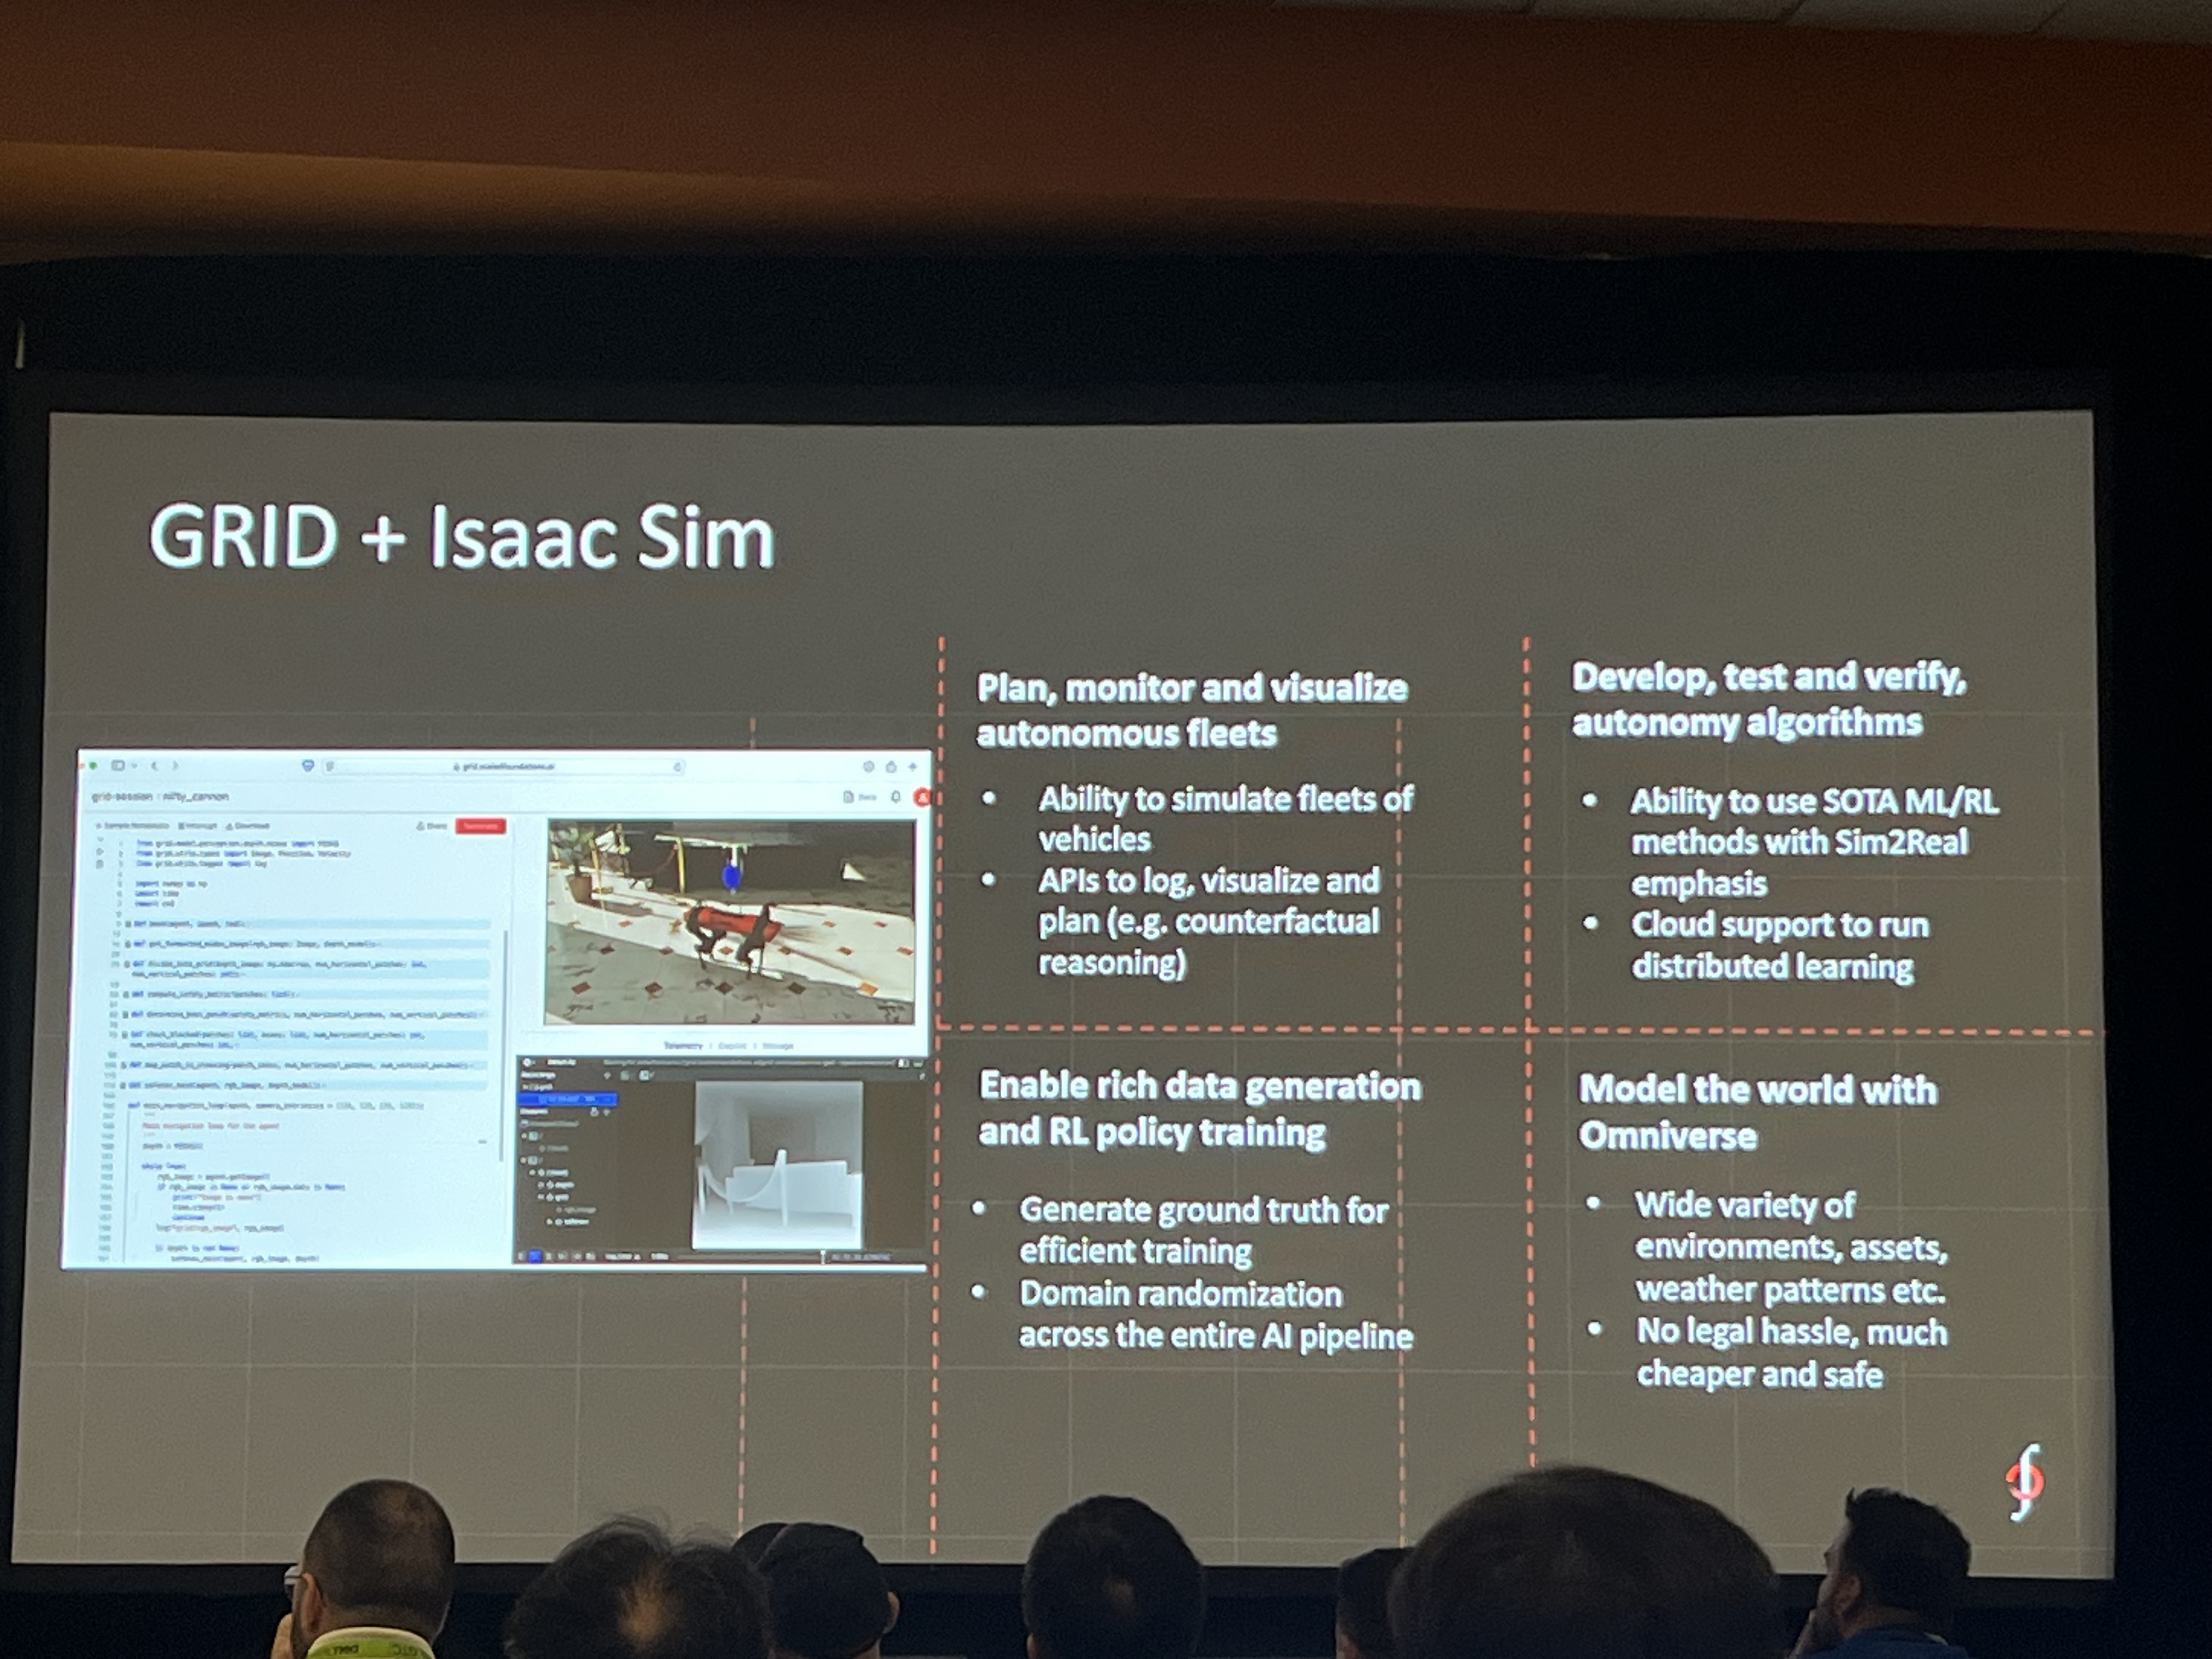
\includegraphics[width=\textwidth]{../images/GRID+sim.png}\\

Grid Platform is like an IDE for building and simulating robots. OpenGrid is a browser-based IDE combining simulation and foundation models with development and deployment layers. 

\section{Hands-on Experience on grid.scaledfoundations.ai}

\end{document}